\section{Problem description and motivation}

The discovery of interstellar objects such as Oumuamua and Borisov within our
solar system has ignited a surge of curiosity and scientific interest. These
sub-kilometer-sized visitors, originating from distant stellar systems, present
a unique opportunity to study extraterrestrial bodies that have traversed vast
cosmic distances. 

Given their exceptionally high eccentricities, heliocentric velocities, and
fleeting passage through the planetary region, there is a pressing need for the
development of ready-to-launch missions capable of intercepting them.

However, the design of such missions is not straightforward. The high velocities
of these objects, combined with their limited observation windows, make it
difficult to accurately predict their trajectories and plan for rendezvous
within the short timeframes available.

The previous problem presents the main motivation of this work: devising
intercepting orbits capable of intercepting interstellar objects. This research
stems from the desire to unlock the mysteries surrounding these enigmatic
interstellar travelers, gathering invaluable data or even returning samples from
their surfaces. This pursuit not only promises to broaden our understanding of
celestial dynamics and planetary formation but also holds profound implications
for the future of space exploration and our comprehension of the broader
universe.

\begin{figure}[H]
  \centering
  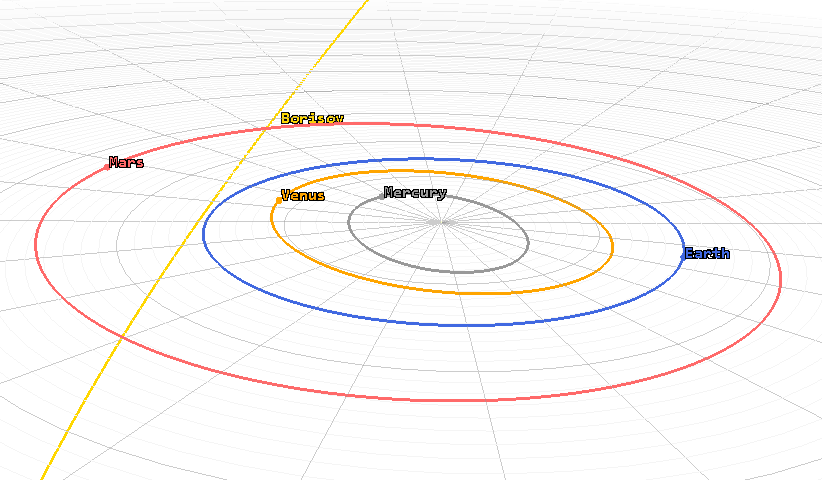
\includegraphics[width=0.95\textwidth]{static/oumuamua/oblique_view.png}
  \caption[Oumuamua orbit through our solar system]{
    Orbit of 1I/'Oumuamua through the solar system. Its eccentricity is
    aproximately $e = 1.20$. This indicates an hyperbolic orbit, meaning that
    Oumuamua is not gravitationally bounded to the Sun. Its high speed and
    trajectory suggest that this body originated from another stellar system.
  }
  \label{fig:oumuamua_orbit}
\end{figure}
